\chapter{Introduction}
\label{chap:introduction} 
\lhead{Chapter \ref{chap:introduction}. \emph{Introduction}}

This chapter presents the general idea of this work. Section~\ref{intro:motivation} describes the motivation for optimization of resource allocation on the cloud. Section~\ref{intro:application} discusses the model of scientific applications. Section~\ref{intro:cloud} describes cloud business models and services that are used to deploy applications. Section~\ref{intro:statement} states the goals of the thesis. Section~\ref{intro:statement} enumerates challenges to be overcomed. 

\section{Motivation}
\label{intro:motivation}

Planning and scheduling activities have been present in people's life ever since first civilization was built. It usually was related to travel planning or construction planning. Ancient romans needed to take care on where aqueducts should be build depending on the demand and how much material should be used. Every craftsman needed to optimize how much material will he use to create his product. Later on, this became event more important during Industrial Revolution.

Nowadays, science requires processing of large amounts of data and use of hosted services for compute-intensive tasks~\cite{Deelman-PPL13}. Cloud services are used not only to provide resources, but also for hosting scientific datasets, as in the case of AWS public datasets~\cite{AWS-public-dataset}. Scientific applications that run on these clouds have often the structure of workflows or workflow ensembles that are groups of inter-related workflows~\cite{Malawski-SC12}. Infrastructure as a Service (IaaS) cloud providers offer services where virtual machine instances differ by performance and price~\cite{Bubak-CCGrid13}. Planning scientific experiments requires optimization decisions that take into account both execution time and cost.

This thesis illustrates typical problems when making decisions on resource allocation for scientific applications on IaaS clouds and how they can be addressed using optimization techniques. In contrast to already well established computing and storage resources (clusters, grids) for the research community, clouds in the form IaaS  platforms (pioneered by Amazon EC2) provide on-demand resource provisioning with a pay-per-use model. These capabilities together with the benefits introduced by virtualization, make clouds attractive to the scientific community~\cite{Deelman09}. As a result, multiple deployment scenarios differing in costs and performance, coupled together with new provisioning models offered by clouds make the problem of resource allocation and capacity planning for scientific applications a challenge.

\section{Scientific applications}
\label{intro:application}

Scientific computing covers a wide range of fields including biology, chemistry, physics, economics, engineering, finance, geophysics, linguistics, mathematics, and mechanics. Applications used in that sciences are often distributed, so that application may run a numbers of magnitude faster than sequential one. This is crucial in some fields such as weather forecasting or financial modelling to get results as fast as possible. 

Scientific applications usually may be put to one of the following groups: 
\begin{itemize}
  \item workflows,
  \item bag of tasks,
  \item map-reduce applications,  
  \item sequential batches,
  \item High Performance Computing applications.
\end{itemize}

In this thesis we will focus on resource allocation for workflows and bag of tasks applications.

\subsection{Workflows}
\label{intro:workflow}

Scientific workflow is concerned with the automation of scientific processes in which tasks are structured based on their control and data dependencies~\cite{Taylor:2006:WES:1196459}. Workflow application is composed by connecting multiple scientific tasks to their dependencies. Workflow structure indicates the temporal relationship between the tasks. In general, a workflow can be represented as a Directed Acyclic Graph (DAG) or a non-DAG. Figure~\ref{fig:intro:workflow} shows example \emph{Montage} workflow that is used to create mosaics of the sky.

\begin{figure}[tb]
   \centering
   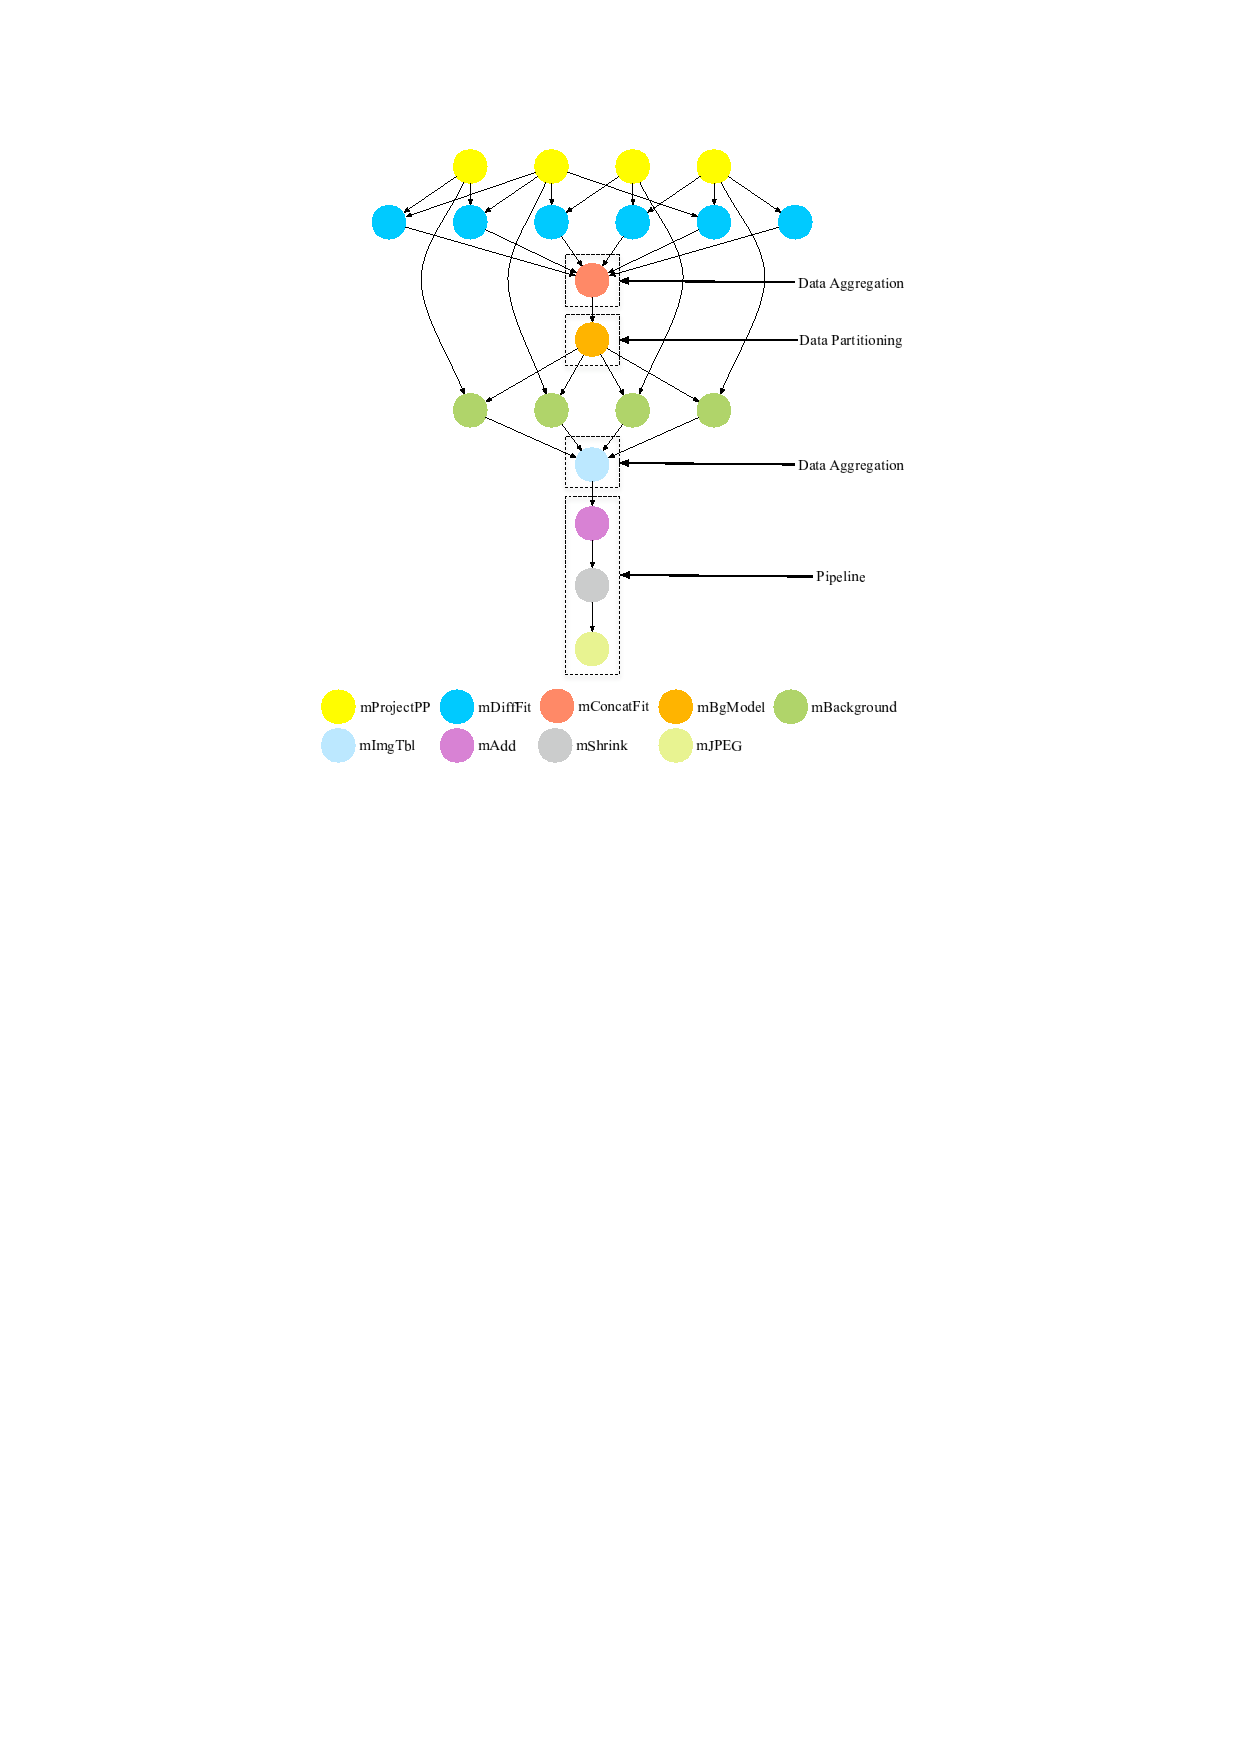
\includegraphics[width=0.7\columnwidth]{MontageWorkflow}  
   \caption{Montage – example workflow~\cite{Bharathi08}}
   \label{fig:intro:workflow}
\end{figure} 


Workflow is built of four base control structures: \emph{sequence}, \emph{parallelism}, \emph{choice} and \emph{loop} (only for non-DAGs). Sequence represents an ordered series of task with one starting after the previous task has completed. Parallelism represents tasks that are performed concurrently, rather than serially. The choice structure allows to run selected portion of the workflow if certain conditions are met. The iteration structure lets certaint block of tasks to be repeated. Consecutive stages of workflow often represent work of scientist – data gathering, preprocessing, processing and results aggregation. 

In terms of scientific computing we will be rather interested in data flow in workflow. It is then composed of the follwing structures (Figure~\ref{fig:intro:workflow:structures}): \emph{process}, \emph{pipeline}, \emph{data distribution}, \emph{data aggregation} and \emph{data redistribution}.

\begin{figure}[tb]
   \centering
   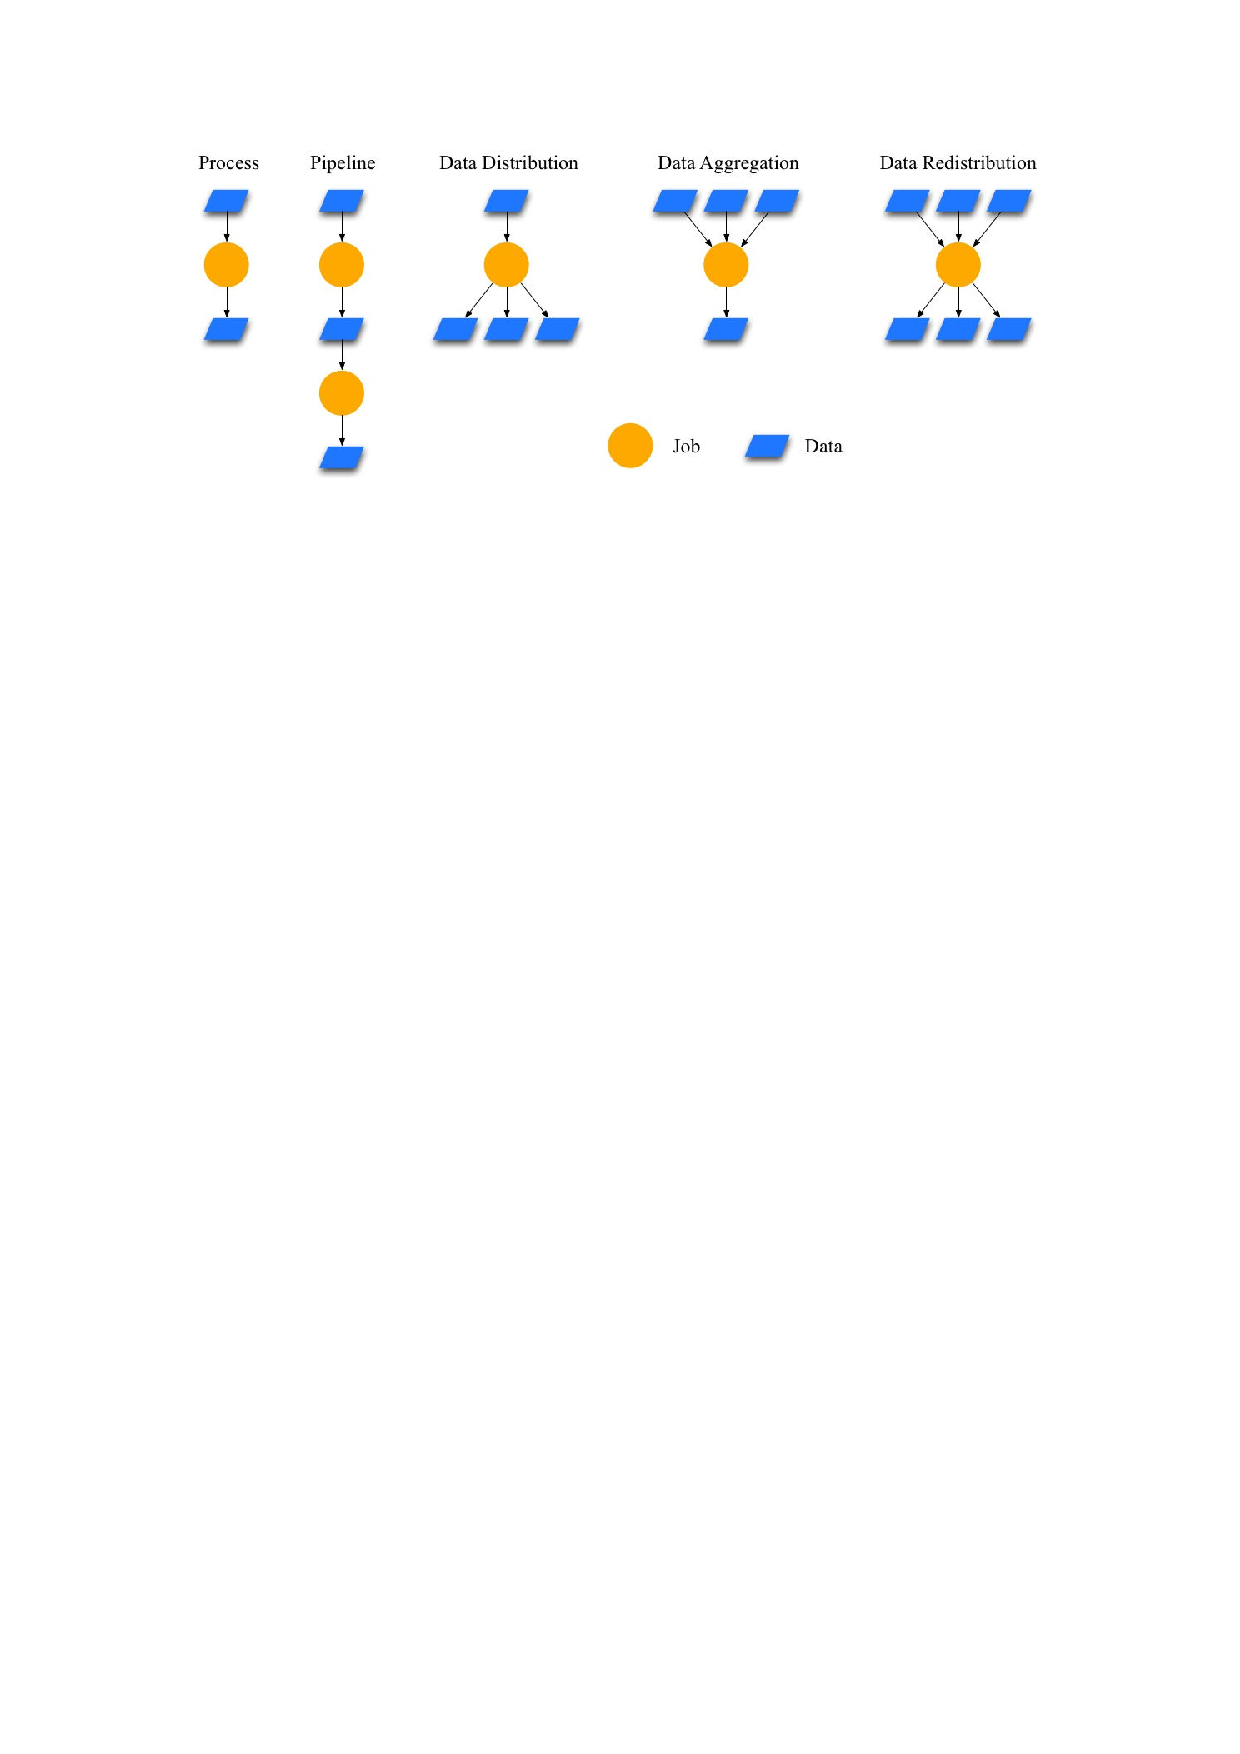
\includegraphics[width=\columnwidth]{WorkflowDataFlow}  
   \caption{Data flow structures in Workflows~\cite{Bharathi08}}
   \label{fig:intro:workflow:structures}
\end{figure} 


Scientific workflows are usually run on shared infrastructure as clusters, grids or clouds. It requires to carefully plan and schedule computation to efficiently use given infrastructure. As the workflows are getting bigger and more complex it is nearly impossible to do it manually. Specifically, scheduling workflow applications in a distributed system is an NP-complete problem~\cite{Garey:1979:CIG:578533}. Example workflow scheduling algorithms are presented in Chapter \ref{chap:state-of-art}.

There exists multiple workflow systems that assist scientists to create and deploy their workflow. Popular ones are Pegasus~\cite{Pegasus} and Taverna~\cite{Taverna}. They provide tools to model workflow either in code or via GUI application. Then one is able to generate workflow execution plan on certain (e.g. grid) architecture. Workflow systems differ in supported workflow types (DAG or non-DAG), workflow scheduling policies and algorithms, fault tolerance, and supported infrastructure. The good overview on workflow systems taxonomy is given in ~\cite{Yu:2005:TSW:1084805.1084814}.

\subsection{Bag of tasks}

Bag of tasks applications represent group of independent tasks that may be processed sequentially or in parallel. There are no dependencies between tasks. A large parameter sweep is good example of such problem. The \emph{map} stage of map-reduce (see Figure~\ref{fig:intro:mapreduce}) application can be also considered as a bag of tasks. Additionally, many workflows include a stages of a high number parallel tasks. Such examples can be found e.g. in typical scientific workflows executed using Pegasus Workflow Management system, where e.g. CyberShake or LIGO workflows have a parallel stage of nearly homogeneous tasks~\cite{Bharathi08}. Other examples are Wien2K and ASTRO workflows that consist of iteratively executed parallel stages comprising homogeneous tasks~\cite{Duan12}. Due to the high number of parallel branches, these stages accumulate the most significant computing time of the whole application, so optimization of the execution of this stage is crucial.


\begin{figure}[tb]
   \centering
   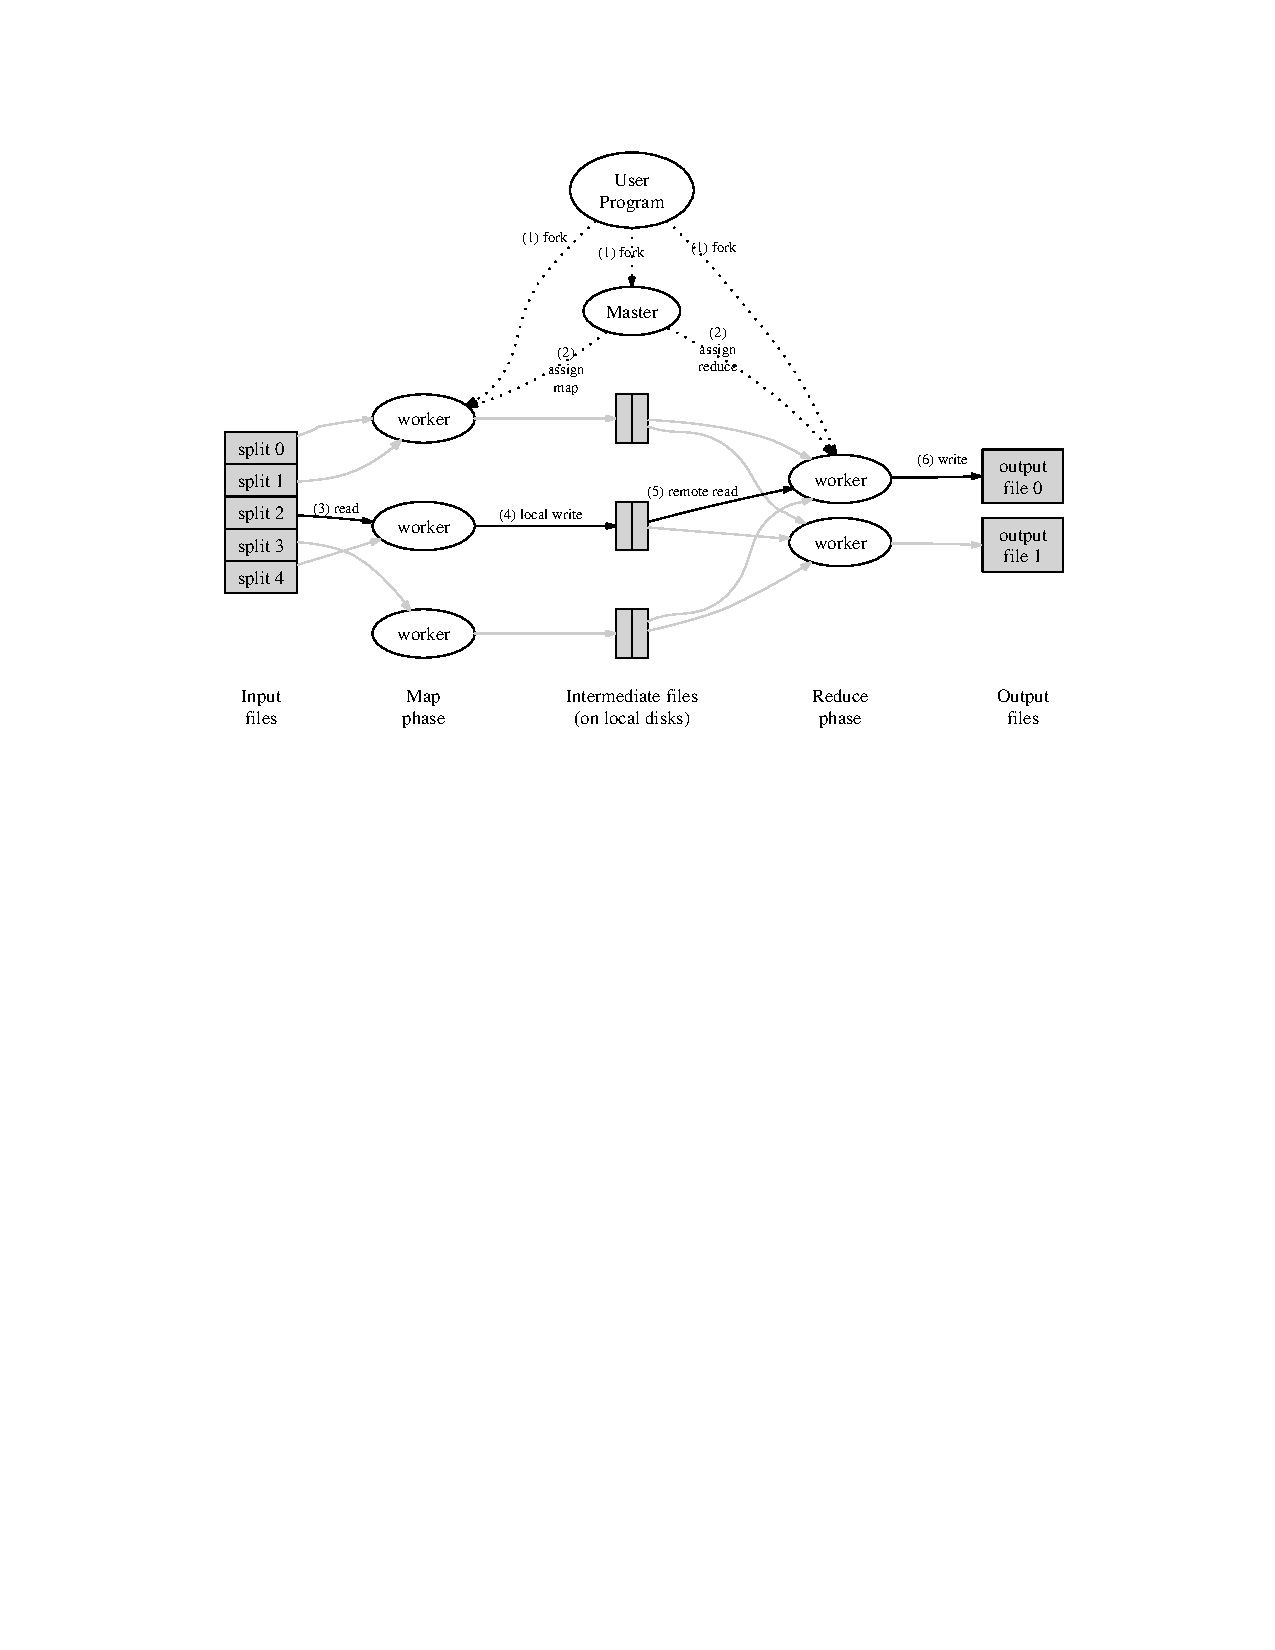
\includegraphics[width=0.7\columnwidth]{MapReduce}  
   \caption{Map-reduce execution overview\cite{Dean:2008:MapReduce}}
   \label{fig:intro:mapreduce}
\end{figure} 


\section{Introduction to Cloud Computing}
\label{intro:cloud}

Cloud computing became de facto standard of delivering computing resources adopted both by commercial and scientific communities. Nowdays, hardly any science can be performed without computational science and cloud systems are regarded by the scientific community as a potentially atractive source of low-cost computing resources as they can be provisioned on-demand according to pay-per-use model.

There are mutliple definitions of the cloud computing. The term is frequently used for marketing of hosted services or applications running in client-server model. As defined by US National Institute of Standards and Technology (NIST)~\cite{NISTCloudDef}, cloud computing is “a model for enabling ubiquitous, convenient, on-demand network access to a shared pool of configurable computing resources (e.g., networks, servers, storage, applications, and services) that can be rapidly provisioned and released with minimal management effort or service provider interaction”.

\subsection{Service models}

We may categorize cloud services in terms of service model that give different level of control and responsibilities to user and service provider:

\begin{description}
  \item[Software as a Service (SaaS).] The capability provided to the user is to use applications deployed by provider running on a cloud infrastructure. The applications are usually available by web-browser based interface or program interface. The underlying cloud infrastructure including network, servers, operating system and application are managed by service provider. Popular SaaS applications include Gmail, Evernote and Salesforce.
  \item[Platform as a Service (PaaS).] The capability provided to the user is to deploy his own appliactions created using programming languages, libraries, services and tools provied by the provider. The consumer does not manage underlying cloud infrastructure including network, servers, operating systems, runtime environment, but has control over the deployed application and configuration settings for cloud enviromnent. Example platforms include Heroku, Google App Engine and Nodejitsu.
  \item[Infrastructure as a Service (IaaS).] The capability provided to the user is to provision processing, storage, networks and other fundamental computing resources where the consumer is able to deploy and run arbitrary software. The consumer does not manage the underlying hardware infrastructure, but has control over operating system, storage, deployed appliations and has possibly limited control over networking (i.e. hosts firewall). Example platforms include Amazon EC2 and Rackspace.
\end{description}

\subsection{Deployment models}

Depending on who manages cloud infrastructure we may distinguish the following models:

\begin{description}
  \item[Private Cloud.] The cloud resources are provisioned for exclusive use by a single organization.
  \item[Community Cloud.] The cloud resources are provisioned for exclusive use by specific community of consumers from organization that have shared concerns. The concept is similar to scientific grid systems.
  \item[Public Cloud.] The cloud resources are provisioned for open use by the general public.
  \item[Hybrid Cloud.] The cloud infrastructure is composed of two or more distinct cloud providers that remain unique entities, but are bound together by technology that enables data and application portability. This technique is used for cloud bursting and offloading peak load to public cloud while using private resources when off-peak times.
\end{description}

\subsection{IaaS compute cloud}

Usually IaaS clouds provide three types of resources that are provisioned with a pay-per-use model: 
\begin{description}
  \item[Computing.] Provided as virtual machine (VM) instances. Multiple instance types are available that differ with CPU power, RAM memory and additional hardware (i.e. GPU units). VMs are usually billed for instance running time (wall clock time, not CPU time) usually rounded up to full hours.
  \item[Storage.] Provided as virtualized disk drives for virtual machines (i.e. Amazon's EBS) or as object store available as external service (i.e. Amazon's S3). User is usually biled for persisting data per GiB\footnote{Gibibyte $= 2^{30}$ bytes} per month. Additional charges may also apply (i.e. per IO transaction).
  \item[Networking.] Provides connectivity between VMs, storages and the Internet. User is billed for the data transfered of the cloud, while incoming data and transfer inside specific cloud usually remains free. Networking is provided in bundle with computing and storage, not as a separate service.
\end{description}

\section{Problem statement}
\label{intro:statement}

In this thesis we will focus on optimization of resource allocation of bag of tasks and workflow applications on the hybrid cloud platforms. Planning scientific experiments requires optimization decisions that take into account both execution time and cost, as well as other constraints. Specifically, we will address the cost optimization problem of large-scale applications running on multiple heterogeneous clouds, using mathematical modeling with AMPL and mixed integer programming.

\section{Goals of the thesis}
\label{intro:goals}

The major goal of this thesis is the theoretical and practical investigation of optimization of resource allocation on the cloud by using integer linear programming tools and methods. The goal will be acomplished by:

\begin{itemize}
  \item study of existing works on workflow scheduling and resource allocation on the cloud,
  \item defining application and infrastructure model,
  \item formulating integer linear problem for bag of tasks applications and workflows,
  \item implementing optimization model in AMPL,
  \item evaluating optimization results, performance and stability,
  \item answering if ILP is suitable method to solve the problem.
\end{itemize}

The goals will be addressed in the following chapters. In Chapter~\ref{chap:state-of-art} we will explore existing work  on scientific application scheduling. In Chapter~\ref{chap:ampl} we will have a quick tutorial on mathematical programming. In Chapters~\ref{chap:bot} and \ref{chap:formulation-workflows} we will go through defining infrastructure and application models that will be then implemented and evaluated. In Chapter~\ref{chap:conclusions} we will answer if ILP is suitable approach for resource allocation on the cloud.
 
\section{Summary}

\todo{Nie klei się}

In this chapter we discussed the motivation an goals of this work. We given a brief overview on scientific applications focusing on bag of tasks applications and workflows. We also introduced cloud computing. We will dive deeper into the IaaS cloud characteristics in Section~\ref{sec:bot:cloudmodel}.

